\section{Non Local Controlflow Repair \cite{AdventureOfALifetime}}
\label{app:non_local_control_flow_repair}

% \begin{algorithm}
%     \caption{FixNonLocalControl}
%     \textbf{Input}: an extracted function EF, an introduced function call expression $E$ (i.e., $EF(...)$) in the caller \\
%     \textbf{Output}: a list of patches PS to apply to the refactored file
%     \begin{algorithmic}[1]
%     \State $PS \gets []$
%     \State $R \gets$ collect return statements in EF
%     \State $B, C \gets$ collect top-level break and continue statements in EF
%     \If{$R \cup B \cup C \neq \emptyset$}
%         \State $RTY \gets BuildReturnType(R, B, C)$
%         \State $PS \gets UpdateReturnType(EF, RTY) :: PS$
%     \For{ $lr \in R$}
%         \State $PS \gets (l_r, return e \rightsquigarrow return Ret(e)) :: PS$ \EndFor
%         \For{ $l_b \in B$}
%             \State $PS \gets (l_b, break \rightsquigarrow return Break) :: PS$
%         \EndFor
%         \For{ $l_c \in C$}
%             \State $PS \gets (l_c, continue \rightsquigarrow return Continue) :: PS$
%         \EndFor
%         \State find location of the final expression of EF
%         \State $PS \gets (l_e, EF(...) \rightsquigarrow ok(E)) :: PS$
%         \State $\bar{CS} \gets BuildCasesForReturnType(RTY)$
%         \State $l_{caller} \gets$ location of E
%         \State $PS \gets (l_{caller}, E \rightsquigarrow match E with C_s) :: PS$
%     \EndIf
%     \State \textbf{return} PS
%     \end{algorithmic}
% \end{algorithm}

\begin{figure*}[h]
    \centering
    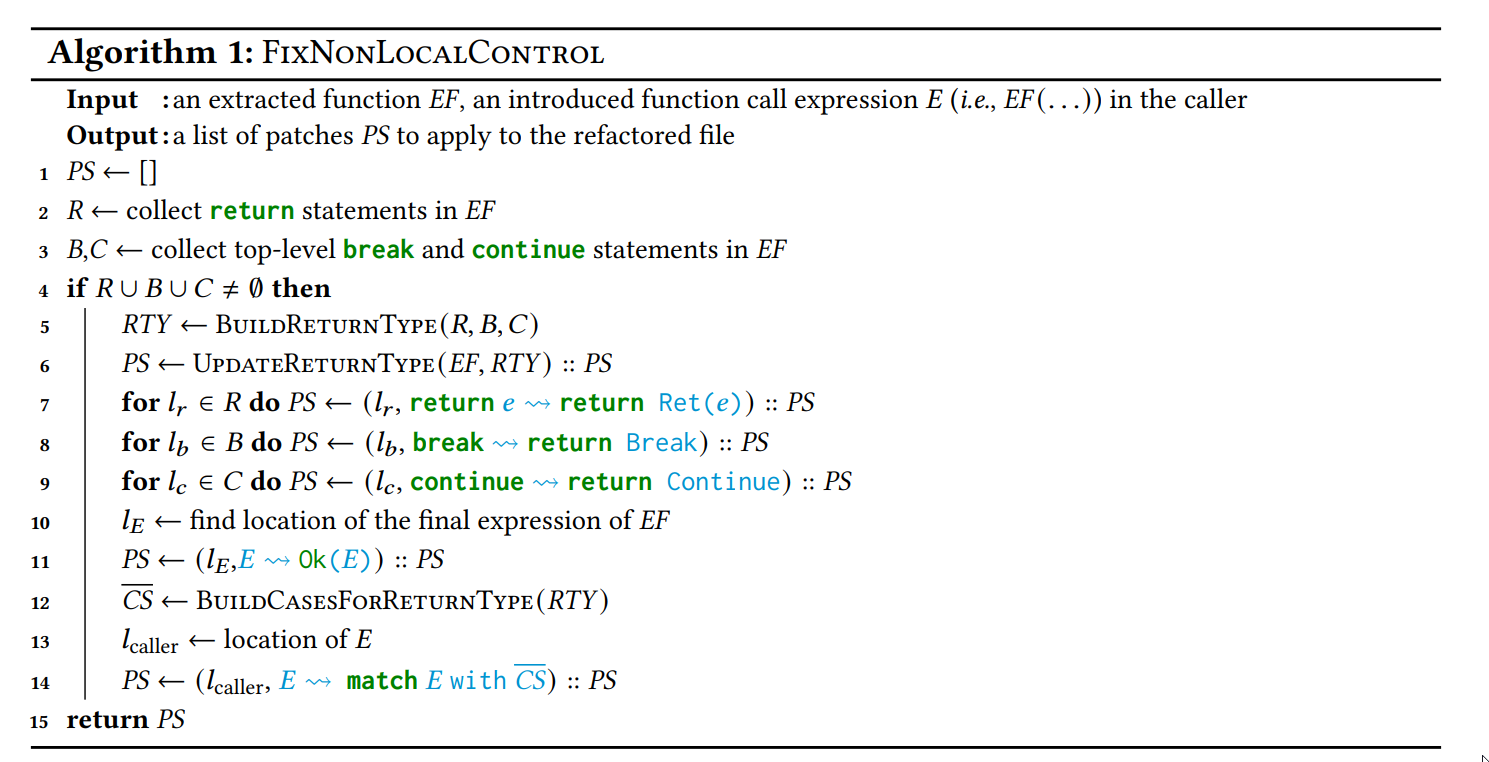
\includegraphics[width=\textwidth]{figures/algo_1.png}
    % \caption{Non Local Control Flow Repair}
    \label{fig:algo_1}
\end{figure*}